\documentclass[a4paper,norsk]{article}
\usepackage{preamble}

\begin{document}
\maketitle

\section*{Mathematical approach}
\begin{align*}
\iint\limits_C \Big(\phi \frac{\partial G}{\partial n} - G\frac{\partial \phi}{\partial n}\Big) dS =
\begin{Bmatrix}
0 \\ \pi \phi(x,y,z) \\ 2\pi \phi (x,y,z)
\end{Bmatrix}
\end{align*}


\begin{align*}
\pi \phi(x_0) = \int\limits_S \Big(\phi \frac{\partial \psi}{\partial n} - \psi \frac{\partial \phi}{\partial n} \Big) dS
\end{align*}

Here $\psi$ = ln r, which is the source potential in 2D. 

\newpage
\section*{Numerical approach}

\begin{align*}
\pi \phi(X_0) + \sum_{n=1}^N \phi(X_n) \int\limits_{Cs} \frac{\partial}{\partial n} ln r \hspace{1mm}dS = 
\sum_{n=1}^N \frac{\partial \phi}{\partial n_{X}} \int\limits_{Cs} ln r \hspace{1mm} dS
\end{align*}


\begin{align*}
\int\limits_{Cs} \frac{\partial}{\partial n_x} ln r \hspace{1mm}dS = -\Big(\theta_B - \theta_A \Big)
\end{align*}

\begin{align*}
\begin{Bmatrix}
\pi \hspace{5mm} (\theta_1 - \theta_2) \hspace{5mm} (\theta_2 - \theta_3) \cdots \\
(\theta_{N-1} - \theta_N)  \hspace{5mm} \pi \hspace{5mm}(\theta_1 - \theta_2) \cdots \\
(\theta_{N-2} - \theta_{N-1})  \hspace{5mm} (\theta_{N-1} - \theta_N) \hspace{5mm} \pi \cdots \\
\vdots 
\end{Bmatrix}
\begin{Bmatrix}
\phi(x_0) \\
\phi(x_1) \\
\phi(x_2) \\
\vdots \\
\phi(x_N)
\end{Bmatrix}
=
\begin{Bmatrix}
\frac{\partial \phi}{\partial n} \int\limits_{C1} ln r_1 \hspace{1mm} dS \\
\frac{\partial \phi}{\partial n} \int\limits_{C2} ln r_2 \hspace{1mm} dS \\
\vdots \\
\frac{\partial \phi}{\partial n} \int\limits_{CN} ln r_N \hspace{1mm} dS
\end{Bmatrix}
\end{align*} 

\begin{figure}[h!]	
	\centering
	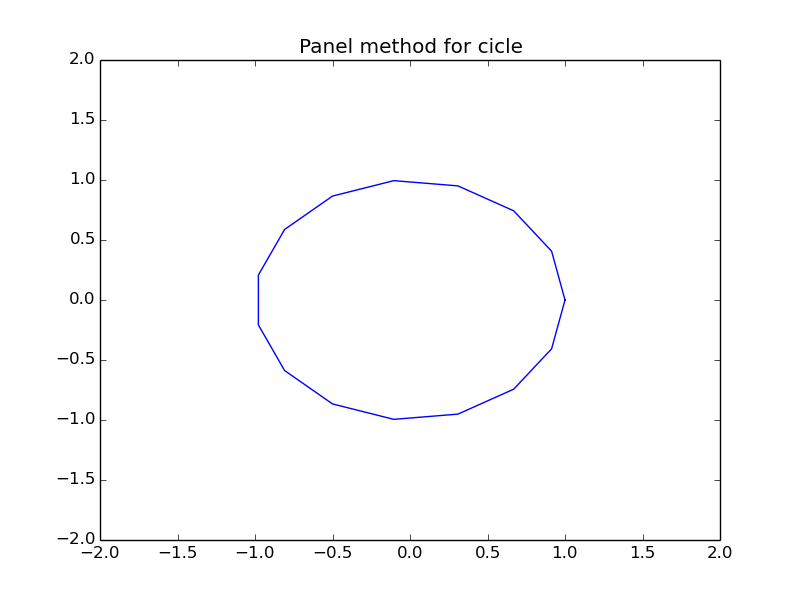
\includegraphics[scale=0.6]{panelcircle.png}
\end{figure}

\newpage
\section*{Results}
Reference solution circle \hspace{2cm} Reference solution ellipse
\begin{itemize}
\item m11: $\rho \pi a^2$   \hspace{3.3cm}    m11: $\rho \pi b^2$
\item m22: $\rho \pi  a^2$  \hspace{3.3cm}    m22: $\rho \pi a^2$
\item m66: 0                \hspace{3.8cm}    m66: $\frac{1}{8}\pi \rho (a^2 - b^2)^2 $  
\end{itemize}

\begin{figure}[h!]	
	\centering
	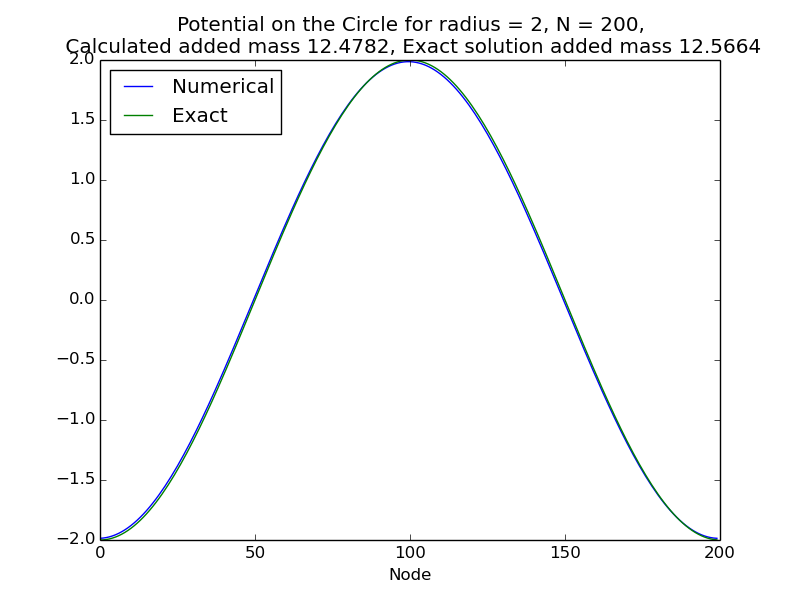
\includegraphics[scale=0.6]{present1.png}
\end{figure}

\newpage
\begin{lstlisting}[style=terminal]

---------------------------BEGIN SIMULATION-----------------------------------------------------

--------------------------- -----CIRCLE-----------------------------------------------------
Radius chosen as 2, with 200 nodes
--------------------------------------------------------------------------------
 For direction 11 Numerical solution 12.478, exact solution 12.566, 
 error 0.993 %
--------------------------------------------------------------------------------
 For direction 22 Numerical solution 12.478, exact solution 12.566, 
 error 0.993 %
--------------------------------------------------------------------------------
 For direction 66 Numerical solution -0.000, exact solution 0.000, 
 error 0.000 %

--------------------------------Ellipse-----------------------------------------------------
Radius r_a = 1, r_b = 3 , with 200 nodes
--------------------------------------------------------------------------------
 For direction 11 Numerical solution 27.882, exact solution 28.274
Error 0.014 %
--------------------------------------------------------------------------------
 For direction 22 Numerical solution 3.127, exact solution 3.142
Error 0.005 %
--------------------------------------------------------------------------------
 For direction 66 Numerical solution 24.655, exact solution 25.133
Error 0.019 %

---------------------------BEGIN SIMULATION-----------------------------------------------------

--------------------------- -----CIRCLE-----------------------------------------------------
Radius chosen as 2, with 400 nodes
--------------------------------------------------------------------------------
 For direction 11 Numerical solution 12.523, exact solution 12.566, 
 error 0.997 %
--------------------------------------------------------------------------------
 For direction 22 Numerical solution 12.523, exact solution 12.566, 
 error 0.997 %
--------------------------------------------------------------------------------
 For direction 66 Numerical solution -0.000, exact solution 0.000, 
 error 0.000 %

--------------------------------Ellipse-----------------------------------------------------
Radius r_a = 1, r_b = 3 , with 400 nodes
--------------------------------------------------------------------------------
 For direction 11 Numerical solution 28.078, exact solution 28.274
Error 0.007 %
--------------------------------------------------------------------------------
 For direction 22 Numerical solution 3.134, exact solution 3.142
Error 0.002 %
--------------------------------------------------------------------------------
 For direction 66 Numerical solution 24.897, exact solution 25.133
Error 0.009 %

\end{lstlisting}


\end{document}